\documentclass[11pt]{article}
\usepackage[utf8]{inputenc}
\usepackage[T1]{fontenc}
\usepackage{geometry}
\usepackage{graphicx}
\usepackage{booktabs}
\usepackage{longtable}
\usepackage{array}
\usepackage{hyperref}
\usepackage{url}
\geometry{margin=1in}

\title{Project Coherent Storage v3: CXL, DPU Offload, and AI/HPC Storage Awareness Architecture}
\author{Project Coherent Storage Working Draft}
\date{May 15, 2026}

\begin{document}
\maketitle

\begin{abstract}
Project Coherent Storage is an inference-first storage architecture in which vLLM and peer inference actors connect only to the Coherence-CE Memory Mesh. Coherence-CE hides lower-layer OpenZFS, DPU, NVMe-oF, RoCEv2, and CXL implementation details while enforcing KV durability classes, placement policy, and scheduler admission. This v3 report updates the v2 ADR set with roadmap evidence for Marvell/XConn CXL, CXL standards, Linux CXL tooling, CXL-enabled KV-cache research, DPU/protocol-offload ecosystems, and arXiv-ready publication workflow. It also defines evidence grades for public roadmap claims so that direct Marvell/XConn CXL evidence is not conflated with adjacent NVIDIA BlueField/STX, Xsight, Broadcom, Pure Storage, IBM, Oracle, or OpenZFS evidence.
\end{abstract}

\section{Architecture Position}
Inference actors do not know about CXL devices, OpenZFS vdevs, DPU queues, RoCEv2 paths, RDMA queue pairs, or NVMe-oF namespaces. They call Coherence-CE through a Coherence-native or OpenAI-compatible API. Coherence-CE owns mapping to GPU HBM, host DRAM, governed CXL T1/T1.5 memory, RDMA object paths, and OpenZFS-backed durability.

\begin{figure}[h]
\centering
\includegraphics[width=0.95\linewidth]{figures/v3-coherence-ce-data-path.png}
\caption{Coherence-CE actor boundary and lower-layer storage path.}
\end{figure}

\section{Audience Tiers}
The rapid-awareness training path separates executive, director, technical ARB, and research-publication questions. Executives focus on memory-wall value, risk, and roadmap timing. Directors focus on procurement, lifecycle, topology, and operational readiness. Technical reviewers focus on data path, failure semantics, scheduler admission, OpenZFS/CXL semantics, and DPU/RDMA qualification.

\begin{figure}[h]
\centering
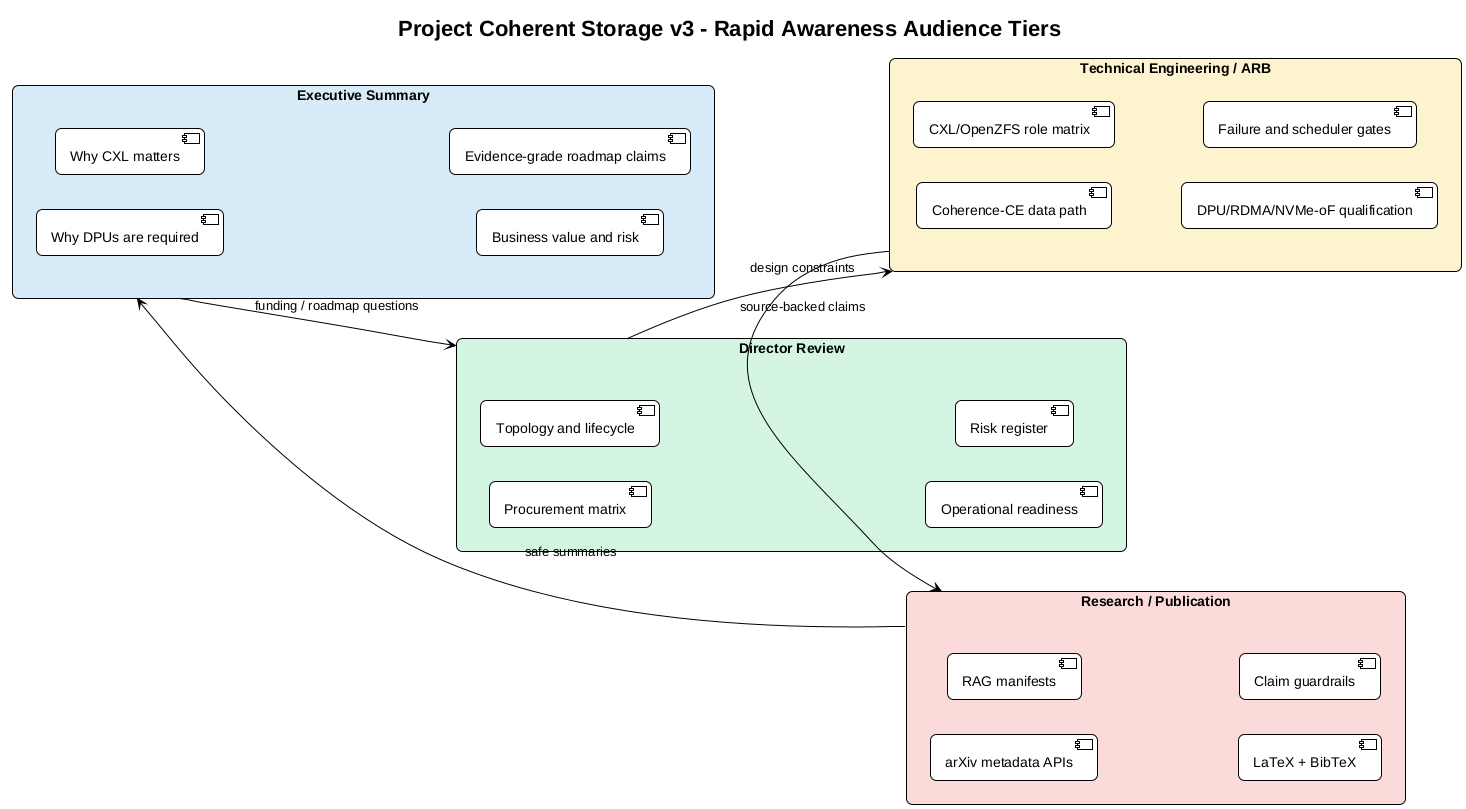
\includegraphics[width=0.95\linewidth]{figures/v3-awareness-tier-map.png}
\caption{Audience tiers for the v3 rapid-awareness training package.}
\end{figure}

\section{CXL Roadmap and Decision Tree}
The v3 evidence set supports CXL as a governed memory expansion and warm/shared memory tier. Marvell Structera and Marvell/XConn public materials support CXL memory expansion, switching, pooling, and interoperability analysis \cite{marvellStructeraS2026,marvellXConnAcquire2026,xconnApollo22025}. CXL 3.1 and 4.0 support statements establish standards-roadmap context \cite{cxl31Support2024,cxl40Support2025}. Linux CXL documentation and ndctl/libcxl provide implementation-readiness references \cite{linuxCXLDocs2026,ndctlLibcxl2026}.

CXL is not automatically local DRAM or durable storage. It is topology-sensitive and must be governed by root-complex locality, NUMA distance, hop count, fabric-manager state, RAS counters, and scheduler-visible telemetry.

\begin{figure}[h]
\centering
\includegraphics[width=0.72\linewidth]{figures/v3-cxl-roadmap-decision-tree.png}
\caption{CXL decision tree for Project Coherent Storage roles.}
\end{figure}

\section{CXL KV-cache and CXL Storage Research}
Recent research strengthens the case for CXL-backed warm KV-cache and CXL-adjacent storage experiments. CXL-enabled processing-near-memory for long-context inference and rack-scale CXL shared KV-cache designs show why Coherence-CE should be able to consider CXL memory as a controlled placement option \cite{kimCXLPNM2025,yoonTraCT2025}. CXL SSD research suggests future block-to-byte and computational-storage directions \cite{kwonCXLSSD2025,yangWIO2026}. These research paths do not change the actor contract: they remain Coherence-owned implementation choices until local p99 latency, failure, security, and scheduler evidence qualifies them.

\section{DPU and Adjacent AI-storage Ecosystems}
DPU/SmartNIC hardware remains a strict requirement for Project Coherent Storage storage-network paths. The v3 corpus retains NVIDIA BlueField/STX, Xsight/Hammerspace, Broadcom, Pure/Marvell NVMe-oF/RoCE, and Marvell NVMe-oF evidence as architecture-relevant sources \cite{nvidiaBlueFieldSTX2026,xsightHammerspace2025,broadcomBCM85667}. These sources are not interchangeable with direct Marvell/XConn+CXL evidence. Public reports must classify them as direct, adjacent, negative-control, or not-found-in-current-sweep.

\section{Evidence-grade Guardrails}
\begin{longtable}{p{0.2\linewidth}p{0.72\linewidth}}
\toprule
Grade & Use in public reports \\
\midrule
Direct & The source explicitly states the relationship, integration, or product capability. \\
Adjacent & The source informs a related architecture path but does not prove the named integration. \\
Negative-control & The source is retained to avoid future conflation or overclaiming. \\
Not found & The current sweep found no direct source-backed mention. \\
\bottomrule
\end{longtable}

\section{Research Metadata and arXiv Preparation}
The v3 package keeps Markdown reports and LaTeX/BibTeX source. arXiv guidance on TeX submission, references, article preparation, and bulk-data access is treated as a publication constraint \cite{arxivSubmitTex,arxivReferencesFAQ,arxivPrep,arxivBulkData}. During this run, the arXiv export API returned HTTP 429 rate-limit responses; the query plan and failures are recorded in the package research directory. Future refreshes should prefer API or bulk-data metadata before adding new PDFs to the RAG corpus.

\begin{figure}[h]
\centering
\includegraphics[width=0.95\linewidth]{figures/v3-arxiv-rag-metadata-workflow.png}
\caption{arXiv and RAG metadata workflow with rate-limit disclosure.}
\end{figure}

\section{Conclusion}
The v3 update makes CXL intent explicit without overstating readiness. CXL expands the architecture's ability to manage warm memory pressure and future pooled memory, while DPUs preserve the storage-network offload boundary and OpenZFS remains the durable NAND substrate. Coherence-CE is the stable API and policy layer that allows these technologies to evolve without leaking hardware complexity to inference actors.

\bibliographystyle{unsrt}
\bibliography{references}

\end{document}
